\section{Machine Learning: tree-based methods}

We now turn out attention to \textit{tree-based methods}, completely different types of statistical methods, both in their setting and the way they operate. We use three major algorithms:

\begin{itemize}
    \item (Simple) Decision Tree
    \item Random Forests
    \item Boosting
\end{itemize}

As for the regressions, we split our database into trimesters, and first fit the models on \texttt{trim=1} data, before using the fitted model for predictions on \texttt{trim=[2,3,4]} observations.

\subsection{Simple Tree}

Following the exact setting we have for regressions (i.e. keeping all variables binary), the initial results we obtain for \textit{accuracy} seem to suggest that the simple tree performs as well but no better than linear or logit regressions, with an average accuracy of 76\%, very close to what we had before.

Behind this result, however, lies a very sharp difference in terms of \textit{prediction}. The simple tree model accurately predicts 91.6\% of true positives, but only 47.5\% of true negatives (recall that, rather confusingly, \texttt{actop\_=1} should be interpreted as \textit{unemployed}). Therefore, in spite of its apparent simplicity, the simple tree is so far the best model if we want to capture active people.

\begin{center}
    \begin{tabular}{lcccc}
        \hline
                           & t1     & t2     & t3     & t4     \\
        \hline
        \texttt{actop\_=0} & 0.9160 & 0.9170 & 0.9169 & 0.9200 \\
        \texttt{actop\_=1} & 0.4898 & 0.4997 & 0.4722 & 0.4803 \\
    \end{tabular}
\end{center}

\subsubsection{Gini Index}
Now, the question we are really trying to answer relates to the marginal effect of each variable, and more generally, to the \textit{relative importance} of each variable. One method which is broadly used for measuring the variables importances is the \textit{Gini index gain per variable}. Recall (from the \textit{Background} section) that the Gini index is defined by:

\begin{equation}
    G = \sum_{k=1}^{K} \hat{p}_{mk}(1-\hat{p}_{mk})
\end{equation}

where $\hat{p}_{mk}$ represents the proportion of training observations in the $m^{th}$ region that are from the $k_{th}$ class.

The Gini index is a measure of the total variance accross the $K$ classes (in our case $K=2$), so in a sense, Gini is an indication of \textit{node purity}. The Gini index takes on small values whenever the probabilities are close to zero or one, that is if the node is \textit{pure}. At each split, we use the variable that maximises the gain in terms of Gini index.

The way to assess a feature's importance is then made easy and relatively straightforward: we simply look at the total amount that the Gini is decreased by due to splits over a given feature (see Figure~\ref{fig:simple_tree_gini}).

\begin{figure}
    \centering
    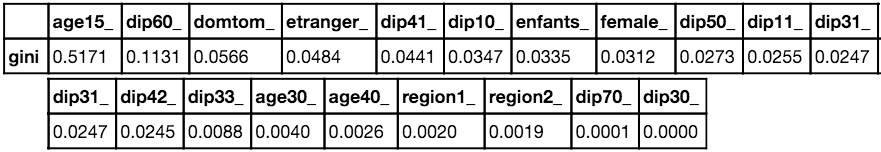
\includegraphics[width=0.8\textwidth]{img/simple_tree_gini.png}
    \caption{Simple Tree --- Gini Feature Importance}
    \label{fig:simple_tree_gini}
\end{figure}

This value gives us an idea of features' importance, and it is also widely used with random forests and boosting methods, because it is easy and computed directly when running the algorithms (that is, without the need to perform more calculations),

\subsubsection{Marginal Effects}
Now that we have an idea of the relative importance of each feature/variable, we would like to measure a more accurate and specific measure of a marginal effect, i.e. what is the effect of a one-unit change in a given variable on the output?

While regressions allowed us to calculate this effect analytically, this is not possible with tree-based methods, so we replicate the "brute force" approach: duplicate the database and modify one parameter from 0 to 1 for everybody, use the fitted model to predict the probabilities for both databases, and take the difference.

We thus obtain a marginal effect per individual and then take the mean marginal effect over all individuals. This gives a good approximation of the marginal effect for the average individual (see Figure~\ref{fig:simple_tree_brute_force}). However, note that the marginal effect of one variable is still dependent on the values of the other parameters.

\begin{figure}
    \centering
    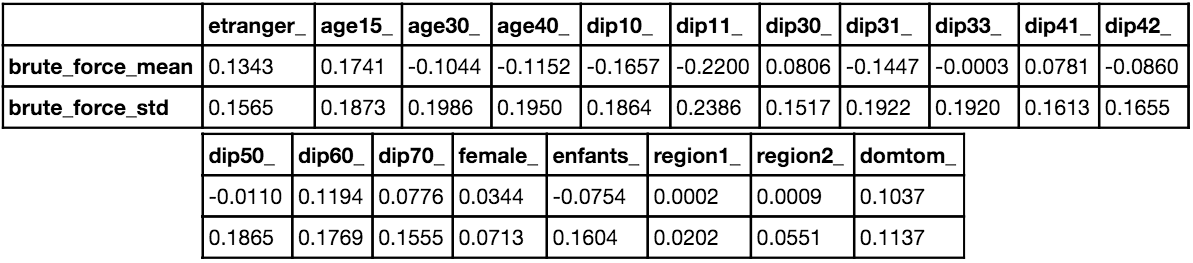
\includegraphics[width=0.8\textwidth]{img/simple_tree_brute_force.png}
    \caption{Simple Tree --- "Brute Force" marginal effects}
    \label{fig:simple_tree_brute_force}
\end{figure}

We observe here that that the parameters with high Gini importance do have a fairly high marginal effect but it is impossible to infer the marginal effect of a change in one variable based only on Gini importance. Gini importance provides a measure of \textit{relative importance} but it is not directly linked with marginal effects.

% TODO(P2): rewrite this section and add a histogram of the distribution of marginal effects for "etranger_" in a simple tree
% Now we are going to have a closer look at those marginal effect.
% First we are going to see what is the importance of the mean value of marginal effect. Indeed, it makes a huge difference if the marginal effects are widespread around the average or on the opposite if the dispersion is really small.
% For that we look at first the standard error of the marginal effect. But this coeficient proved not to be enough, we would need to use a study of the skewness and the kurtosis. So what we opted for is simply studying the distribution itself of those marginal effect.
% Here is an example of the distribution of the marginal effect of being a foreigner.

% TODO(P2): what is this?!
% We found a huge quantity of individuals for whom the marginal effect is simply zero. It means that the variable "etranger\_"has been used as a split in their way down to the last node (or simply that the individual was a foreigner in the previous database already).
% Thus we have a fair vision of the marginal effect of a variable.

With the "brute force" method, we find a mean value and a standard deviation. This standard deviation measures the dispersion of the marginal effect across individuals, and is in fact not the dispersion we are looking for. What we would like is to build a 95\% confidence interval for the value of the mean marginal effect.

In order to find this, we use the \textit{bootstrap} method, which consists in the following procedure repeated $n$ times (see results in Figure~\ref{fig:simple_tree_bootstrap}):

\begin{enumerate}
    \item Create a "new" dataset by picking observations from the original dataset \textit{with replacement}
    \item Compute the mean marginal effect for each variable in the new dataset
    \item Construct the interval by excluding the 2.5\% smallest/largest values
\end{enumerate}

We used $n$ = 1000 for simple trees, but for later methods (e.g. boosting), we had to reduce this value to limit computation time.

\begin{figure}
    \centering
    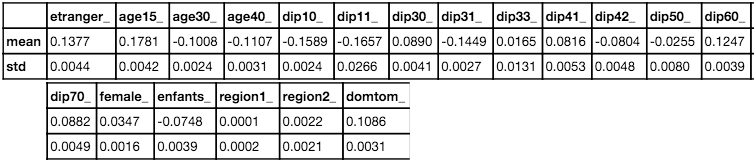
\includegraphics[width=0.8\textwidth]{img/simple_tree_bootstrap.png}
    \caption{Simple Tree --- 95\% confidence interval for mean marginal effects ("Bootstrap")}
    \label{fig:simple_tree_bootstrap}
\end{figure}

The results we obtained for a simple tree are relatively satisfying --- it is easy to infer a sense of causality in the model.

At the same time, it is clear that the simple tree is limited. The quality of the predictions are not any better in our case and don't justify the computation time spent calculating the marginal effects. However, simple trees classify the individual in a very different way than regression methods and even though it is a relatively simple method, it will still fit better to certain classes of problems. As a result, growing a tree or two to see how they fit the data should be done most of the time.

In order to exploit the nature of the tree better, we also tried to grow a tree directly using categorical variables (as opposed to converting all variables to a set of binary variables), as long as the variables could be ordered. We did obtain slightly better result on average (77.5\% accuracy) but the most striking part was that we predicted the people who are active (i.e. \texttt{actop\_=0}) even better, 93\% of the time.


\subsection{Random Forests}

We will not expand here on how random forests work --- we point the reader to the theory in \textit{Background}. However, it is important to point out that the random forest algorithm is an aggregation of simple trees, and that it is expected to improve prediction quality by introducing some randomness.

In our very specific case, with only a few independent variables to choose from, all of which are binary or categorical, the prediction accuracy we get is rather disappointing when compared with the complexity of the algorithm: the overall accuracy we can reach is below 78\%, a result similar to what we get with a simple tree.

However, using (the original) categorical variables for \texttt{age} and \texttt{diploma} instead of binary variables, and using a maximum depth of tree of 9 and a maximum feature per tree of 5, we managed to reach a 93.5\% accuracy for prediction of active people, the best we’ve found so far. The cost of this improved accuracy is that we are below 50\% for predicting inactive people (approximately 46\% over the four quarters).

The results we obtain here are somewhat disappointing --- nevertheless, we would like to emphasise that this we believe this to be mainly due to our setting. In general, random forests do give better predictions than simple trees, but as the algorithm is still based on simple trees, it is expected to conserve some its the main features.

\subsubsection{Gini index}
We used the exact same methods to calculate Gini importance as for simple trees. We expect to find some similarities between the Gini index with simple trees and random forests --- at the very least, we expect the least important parameters in the simple tree to be more important in random forests due to the randomisation of the choice of independent variables (see Figure~\ref{fig:random_forest_gini}).

\begin{figure}
    \centering
    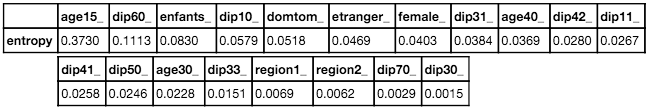
\includegraphics[width=0.8\textwidth]{img/random_forest_gini.png}
    \caption{Random Forests --- Gini Feature Importance}
    \label{fig:random_forest_gini}
\end{figure}

As we can see the main features are still the same even though the values vary a little bit. The gap between the most important and the least important variables is smaller, and a few small changes have occured but overall values are somewhat comparable.

\subsubsection{Marginal Effects}

We now take a closer at the real mean marginal effects, computed empirically. We expect to find some relationship between the results found for simple tree and and those we have now obtained.

\begin{figure}
    \centering
    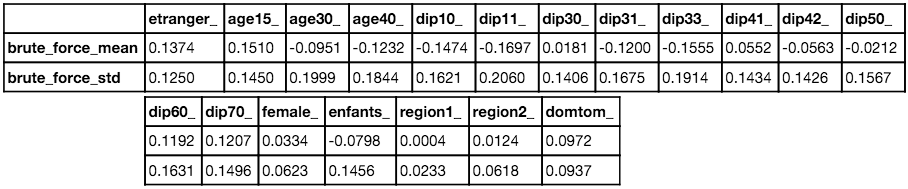
\includegraphics[width=0.8\textwidth]{img/random_forest_brute_force.png}
    \caption{Random Forests --- "Brute Force" marginal effects}
    \label{fig:random_forest_brute_force}
\end{figure}

As we can see here, the marginal effect of \texttt{dip11\_} (highest degree of education) is largest in absolute value, however \texttt{dip11\_} is not very important in terms of its Gini index, which means that it wasn't significant in terms of purity gain. One reason could actually be that because few people have \texttt{dip11\_}, using it at a split at the very beginning does not produce a later gain in purity compared to other variable such as \texttt{age15\_} for instance. As a result \texttt{dip11\_} is only used as a very late split and so its purity gain may be regarded as somewhat negligible.

This actually emphasises the point we already made earlier about the simple tree. The Gini index is somewhat interesting for its simplicity but it only gives us an idea about relative marginal effects and it is only relevant when the dataset of people with the two features are approximately of the same size.

As for the mean marginal effect values we obtained,  we can emphasise once again that the values are very different across parameters, both in terms of sign or magnitude. This means that it is somewhat easy to deduce a relevant sense of causality from these values, i.e. we can picture what feature is important in the prediction we make for a given individual.

In order to give some statistical foundations to our mean marginal effects, we also used the bootstrap method (with $n=1000$ iterations) to calculate a 95\% Confidence Interval (see Figure~\ref{fig:random_forest_bootstrap}). Note that while this computation was relatively fast for simple trees (3.5 seconds per iteration), it was much slower for the random forest (4 minutes per iteration), due to the nature of the algorithm.

\begin{figure}
    \centering
    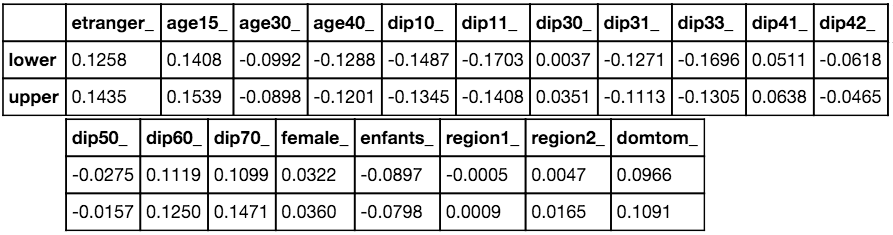
\includegraphics[width=0.8\textwidth]{img/random_forest_bootstrap.png}
    \caption{Random Forests --- 95\% confidence interval for mean marginal effects ("Bootstrap")}
    \label{fig:random_forest_bootstrap}
\end{figure}

% Once we have such interval, given the dispersion of the marginal effects around the average which is very spread it is really interesting to have a deeper look at the distribution of the marginal effect around the mean. For that we just infer it from the duplication of the DataBase, but it could be interesting to  reinforce the relevance of such values by using Bootstrap but again, a look at the time it costs makes it hard to complete.

% TODO(P2): rewrite this section + distribution by histogram of age15, dip11, etranger
% The distributions highlight the fact that the marginal effects are really dependent on the values of other parameters. But still, with all we have gotten, it does seem like we can figure causility in Random Forest almost as well as in Logistic Regression, the only big trouble is the computation it requires. Especially, if we want to have a good accuracy of any marginal effect, that is for any new given individual we could compute the gain/loss of having such feature or not, we would need huge DataBase information so we could be able to assess it. Such a huge DataBase would in turn need a great deal of time to be processed. As a consequence, the more precision we want, the more data and time we need. That is a huge downer compare to a Logit wherein marginal effects can be computed directly and straighforwardly. We found that even in the case of binary variable (non continuous), the mathematical formula is still pretty accurate.
% The last thing we would like to focus on is the Odds-ratios. That is, the odds given a certain feature divided by the odds for the reference average individual.

\subsubsection{Odds Ratios}
As we did for the logit method, we also calculate odds ratios (see Figure~\ref{fig:random_forest_odds_ratios}), using the following formula:

\begin{equation}
    OR = \frac{P(y=1|x=1, X_{-1})/P(y=0|x=1, X_{-1})}{P(y=1|x=0, X_{-1})/P(y=0|x=0, X_{-1})}
\end{equation}

Recall that an odds ratio close to 1 means that the variable doesn’t add a lot of information. If it is close to zero, it means the variable strongly increases the probability that the individual works, and a ratio far beyond one indicates the opposite.

\begin{figure}
    \centering
    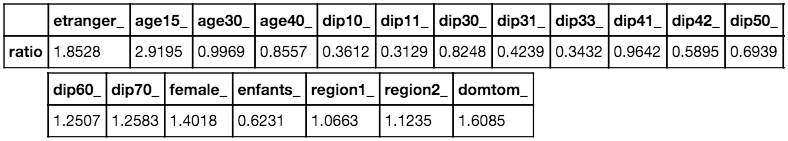
\includegraphics[width=0.8\textwidth]{img/random_forest_odds_ratios.png}
    \caption{Random Forests --- Odds Ratios}
    \label{fig:random_forest_odds_ratios}
\end{figure}

It is important to notice that in some cases, we did find a high mean marginal effect but in the particular case where we look at the reference individual the marginal effect is neglectable. This is the case for instance with \texttt{age30\_} --- which means that for an individual, being in his/her 30s is very similar in terms of prediction to being in his/her 50s (the reference variable).

Another interesting point is that odds ratios are easily compared between models. Unsurprisingly, we find that the ratios are very similar between the simple tree and the random forest, slightly less spread out in the case of the random forest. This makes sense when we think about the random forest algorithm, since a variable that may not be used much in a single tree may take more importance when it comes to the random forest due to the randomisation of predictors' selection.

We find that it is indeed possible to infer causality with the random forest algorithm, and to assess the importance of each predictor according to other predictor values. The main limits of this approach are the computation time and the amount of data that are required to find interesting results. However, assuming we have access to large datasets and very powerful machines, it would make sense to use random forests if the prediction it makes is more accurate.

Given that the functional form (e.g. logit) and tree-based approaches are very different, random forest will prove better than any regression in many cases, and it should not be ruled out because it lacks a (direct) sense of causality. Indeed, if it is needed and worth it, causality is computable.


\subsection{Boosting}
As our last Machine Learning algorithm pick, we opted for boosting --- we used the AdaBoost algorithm available in \texttt{scikit-learn}, and took a simple tree as a base estimator.

The first aspect of boosting we would like to emphasise is that it is a relatively complex algorithm. Indeed, the fact that the computation of each new tree relies on the previous trees makes it impossible to parallelise fully, which means that computation time is very long. In contrast, with random forest, we can take advantage of large multi-core machines to speed up the computation, which is impossible with boosting.

The results we obtained for boosting are somewhat disappointing. The prediction is hardly any better than what we would obtain with a logistic regression. The general prediction accuracy is around 78\%. Once again, the algorithm is very good at predicting $1$’s (\textasciitilde91,5\%) but not very good at predicting $0$’s (\textasciitilde52\%). As the boosting algorithm is also based on simple trees, it makes sense that we find once again, the main characteristics of the simple tree we grew earlier, especially considering we used the very same predictors.

However disappointing the results, in many cases, boosting algorithms outperform all the other models we have applied. The fact that this does not happen in this specific situation is not a contradiction. Our model is very specific with only binary variables and we do not possess enough informative variable to truly make a difference.

With that being said, it is still relevant to see (1) whether the marginal effects we obtained are relevant, (2) how can we make them statistically significant, and (3) how can we interpret and use them to infer the hidden causality relationships.

\subsubsection{Marginal Effects}
We have applied to this model, the very same methods as before in order to find out marginal effects per variable. The results can be found in Figure~\ref{fig:boosting_brute_force}.

\begin{figure}
    \centering
    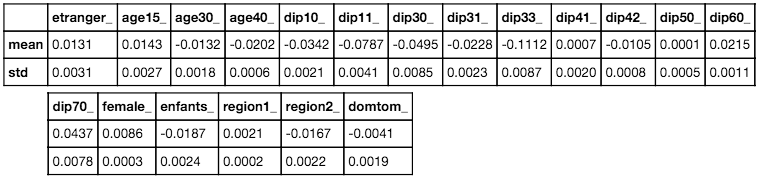
\includegraphics[width=0.8\textwidth]{img/boosting_brute_force.png}
    \caption{Boosting --- "Brute Force" marginal effects}
    \label{fig:boosting_brute_force}
\end{figure}

We first notice that the absolute values we obtain are very small, which means that that the marginal effects seem less spread towards extreme values. The dispersion around the mean is still very consequent but the means themselves are much smaller than what we obtained for random forests or simple trees for instance.

A plausible explanation for this can be found by looking more closely at the algorithm itself. Boosting grows trees recursively and based on previous trees' residuals --- then, it makes sense to infer that more variables are involved in the prediction process and especially that the most important variables (in previous models) would lose some of their dominance. As a result, boosting seems to "even out" the impact of each variable.

% TODO(P2): rewrite this section + histogramme effet marginal de dip11_
% We can of course still denote some differences, for instance dip11 has on average the biggest impact on the final prediction. Here is the distribution of the marginal effects around the mean :

% The distribution is very important to understand how it works indeed. Some variable could have opposite marginal effect depending on some other features so it important to try to perceive those.
% So far I did not mention the Gini index importance (or entropy since we used entropy as our purity estimator) because actually in this specific case the weaknesses of that notions are simply too striking. In the case of boosting, founding any sensible reasoning upon those figures would be very misleading if we compare to the real impact (marginal effect) the predictors have. So, we suggested not to rely on those figures before, in this setting we would warmly recommend not to infer causality using such results.

In order to ensure that the means we found are statistically significant, we also computed a 95\% confidence interval using the bootstrap method. It is important to note however, that due to the nature and complexity of the boosting algorithm, we were not able to run more than $n=500$ iterations, and that even by limiting the number of iterations, the computation took more than 30 hours in total and required very large amounts of memory.

\begin{figure}
    \centering
    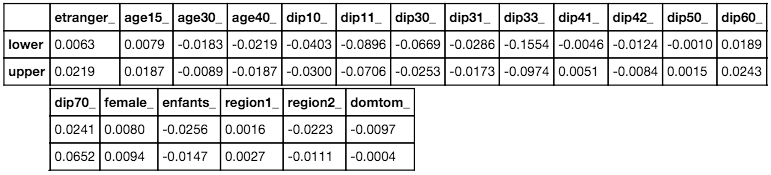
\includegraphics[width=0.8\textwidth]{img/boosting_bootstrap.png}
    \caption{Boosting --- 95\% confidence interval for mean marginal effects ("Bootstrap")}
    \label{fig:boosting_bootstrap}
\end{figure}

This is a very important limit of the boosting model --- because of the great amount of computation required, it is difficult to practice "trial-and-error" and thus, the boosting algorithm is less interesting than other methods.

\subsubsection{Odds Ratios}
Finally, we take a quick look at the odds ratios for the boosting model (Figure~\ref{fig:boosting_odds_ratios}. As expected, we find that the odds ratios are as spread out as before, and this reinforces the general idea that marginal effects are less distinct than before and that they range within smaller absolute values, leading in turn to odds ratios that are closer to $1$.

\begin{figure}
    \centering
    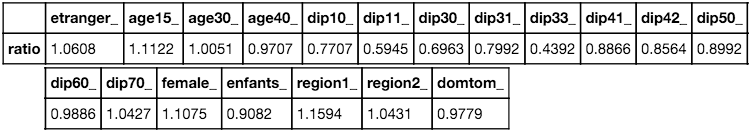
\includegraphics[width=0.8\textwidth]{img/boosting_odds_ratios.png}
    \caption{Boosting --- Odds Ratios}
    \label{fig:boosting_odds_ratios}
\end{figure}

This is an interesting distinction between random forest and boosting, which seems to indicate that boosting trie to look at the "bigger picture" of an individual's characteristics, while random forests give more importance to the main characteristics.
